\chapter{Text mining in Climate, Marine and Environmental Science}

\todo[inline]{Text mining work in related areas, e.g. Kyoto, GeoDeepDive, text mining for Marine Ecological Genomics, environmental QA in machine reading challenge}

Text mining of scientific literature, and literature-based knowledge discovery in particular, has its roots in biomedicine.
Research has matured to a level that text mining applications and services have started to be really helpful to researchers in biomedicine.
Although biomedicine is still by far the most popular application domain, literature mining is now gradually spreading out to other scientific fields.
Yet, despite our best efforts in searching the literature, published work on text mining in climate, marine or environmental science turned out to be extremely rare.
On the one hand, this is unfortunate, because it means there is almost no prior work in our domain of interest that we can build on.
On the other hand, it indicates that the work on literature-based discovery in Ocean-Certain is pushing the limits and holds potential for delivering new and interesting results.

Given the lack of prior art, this chapter surveys work in fields outside biomedicine but related to Ocean-Certain, in fields such as chemistry, geology and ecology.
The first part desribes tools and resources, whereas the second part addresses complete systems. 

\section{Tools and Resources}

\subsection{Vocabularies , Taxonomies and Ontologies}

There are several specialized controlled vocabularies and ontologies which may benefit text mining in climate, marine and environmental science.
 
The Environment Ontology\footnote{\url{http://environmentontology.org/home}} (EnvO) is an ontology about environments  \citep{Buttigieg2013Environment} of biological organisms.
It provides a controlled, structured vocabulary of over 1800 terms to annotate biological entities or samples with environmental descriptors.
There are three main types of terms:

\begin{itemize}
\item \emph{biome}: e.g., boreal moist forest biome, tropical rain forest biome, and oceanic pelagic zone biome 
\item \emph{environmental feature}: e.g, mountain, pond, whale fall, and karst
\item \emph{environmental material}: e.g., sediment, soil, water, and air
\end{itemize}

\noindent The ontology is intended to facilitate integration, archiving and federated searching of environmental data.
It also contains environmental terms in the domain marine biology.
For example, Figure~\ref{fig:envo-example} shows the term \emph{marine algal bloom}.
The left side shows a definiton, known synonymyms (\emph{red tide}), and links to external definitions like the one in Wikipedia.
The right side shows a graphical representation of the ontological relations.
For instance, that \emph{marine algal bloom} is a kind of \emph{algal bloom}, which ultimately is a kind of \emph{environmental feature}, and that  \emph{marine algal bloom} is located in a\emph{ marine biome}, which ultimately is an \emph{environmental system.}

\begin{figure}
\begin{center}
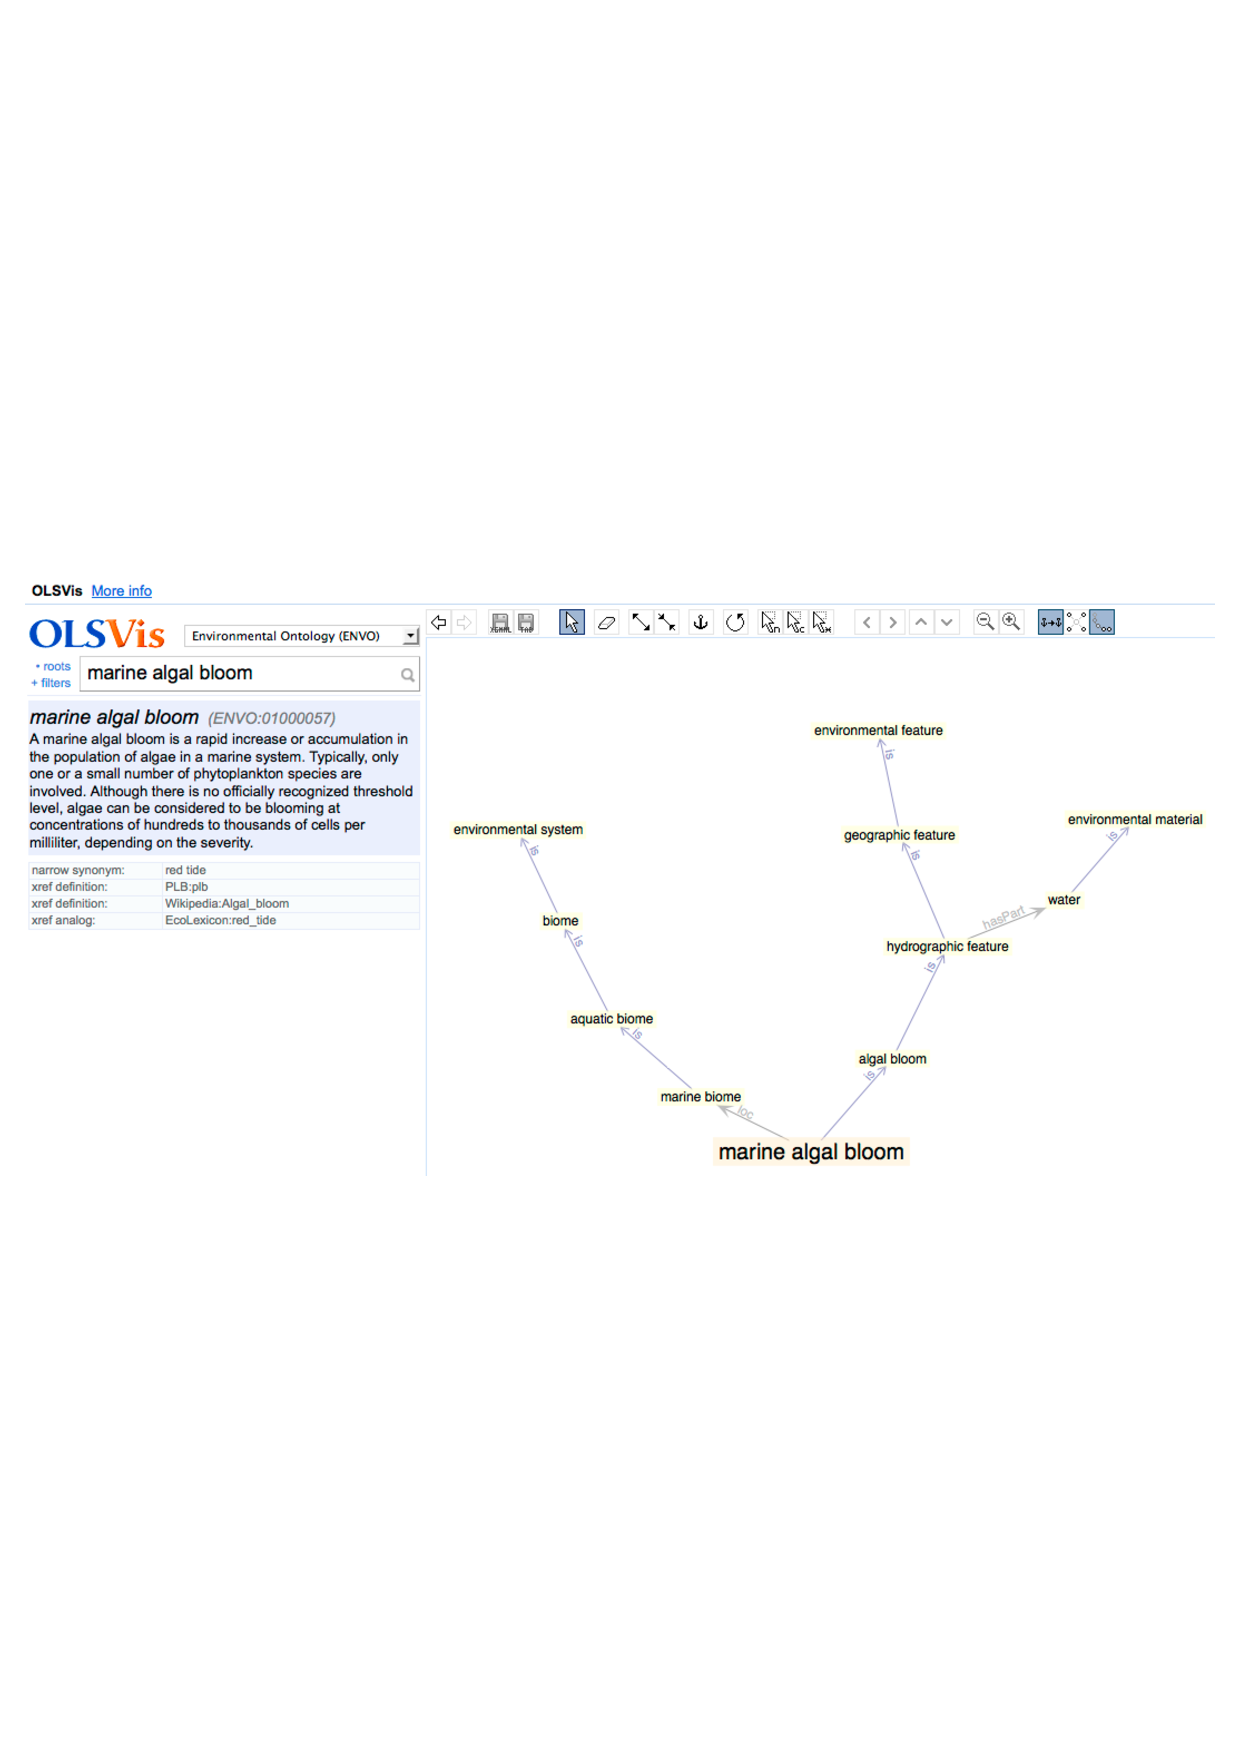
\includegraphics[scale=0.6]{figures/envo-example.pdf}
 \caption{Example of entity \emph{marine algal bloom} in EnvO ontology}
\label{fig:envo-example}
\end{center}
\end{figure}


WoRMS\footnote{\url{http://www.marinespecies.org/}}  (World Register of Marine Species) aims to provide an authoritative and comprehensive list of names of marine organisms, including information on synonymy \citep{Costello2013Global}.
It contains over 220 thousand species, with an estmated coverage of over 95\%.
There is a webservice for tasks such getting the full classification for your taxa, resolving unaccepted names to accepted ones or resolving a common name to a scientific name.

The Marine Metadata Interoperability\footnote{\url{https://marinemetadata.org/}} (MMI) project has as its mission promoting the exchange, integration and use of marine data through enhanced data publishing, discovery, documentation and accessibility.
It hosts, among other things, an ontology repository and associated semantic framework that can be used by the marine science community to store, manage, and work with its scientific vocabularies.

\subsection{Named Entity Taggers}

Many named entity taggers are developed for biomedicine and target specific entities of interest in this domain, such a proteins, genes and drugs.
These are of limited use for text mining in climate, marine and environmental science. 
However, there are a number of taggers for recognition and normalization of biological or chemical entities that are potentially useful for our purposes.

LINNAEUS\footnote{\url{http://linnaeus.sourceforge.net/}} is an open-source software package for species name recognition and normalization \citep{Gerner2010LINNAEUS}. 
Enities are normalized by linking them to unique indentifiers the NCBI taxonomy database\footnote{\url{http://www.ncbi.nlm.nih.gov/taxonomy}}, a curated classification and nomenclature for all of the organisms in the public sequence databases, covering about 10\% of the described species of life on the planet.
It uses a dictionary-based approach to identify species names and a set of heuristics to resolve ambiguous mentions, obtaining 94\% recall and 97\% precision on entity recognition, with 97\% of all mentions resolved to the correct NCBI taxonomy identifiers.
 
The SPECIES (Identification of Taxonomic Mentions in Text) project\footnote{\url{http://species.jensenlab.org/}} has developed taggers for species and organism mentions in text \citep{Pafilis2013SPECIES}. 
The taggers allow for both identification of names in the text and normalization to the corresponding entries in the NCBI taxonomy.
These tools are claimed to be an order of magnitude faster than LINNAEUS.

OSCAR4\footnote{\url{https://bitbucket.org/wwmm/oscar4}} (Open Source Chemistry Analysis Routines) is an open source extensible system for the automated annotation of chemistry in scientific articles \citep{Jessop2011OSCAR4}.
It can be used to identify chemical names, reaction names, ontology terms, enzymes and chemical prefixes and adjectives, and chemical data such as state, yield, IR, NMR and mass spectra and elemental analyses. 
In addition, where possible, any chemical names detected will be annotated with structures derived either by lookup, or name-to-structure parsing using OPSIN or with identifiers from the ChEBI (Chemical Entities of Biological Interest) ontology.

ChemSpot\footnote{\url{https://www.informatik.hu-berlin.de/forschung/gebiete/wbi/resources/chemspot/chemspot/}} is another set of tools for named entity recognition and classification of chemicals in texts, including trivial names, abbreviations, molecular formulas and International Union of Pure and Applied Chemistry (IUPAC) chemical compounds. 
ChemSpot employs supervised-machine learning (Conditional Random Fields) and a dictionary, as well as pattern-based recognition, a classifier model and several methods for consolidating all annotations. 
ChemSpot also performs entity normalization by assigning identifiers from numerous chemical databases. 

CheNER\footnote{\url{http://chener.bioinfo.cnio.es/}} (Chemical Named Entity Recognizer) is another recent tool. It specializes in processing IUPAC entities, on which it is shown to outperform Chemspot \citep{Usie2014CheNER}.

The ENVIRONMENTS\footnote{\url{http://envo.her.hcmr.gr/environments.html}} (Identification of Environment Descriptive Terms in Text) project aims to produce software identifying environment descriptive terms in text, such as \emph{coral reef}, \emph{cultivated land}, \emph{glacier}, \emph{pelagic}, \emph{forest} or \emph{lagoon}.
It allows for orthographic variation in the way the terms are written (e.g. plural forms and spacing/hyphenation like in freshwater, fresh-water, and "fresh water).
Terms are normalized by linking them to a unique identifier is the Environmental Ontology (EnvO).
The project is ongoing and as of yet no software has been released.

\section{Text Mining Systems}

EnvMine is a text-mining system in the field of microbial ecology that automatically extracts contextual information from text like published articles or web pages \cite{Tamames2010EnvMine}.
The motivation is that in ecological studies, it is crucial to have adequate descriptions of the environments and samples being studied. 
Two types of contextual information about sampling sites are targeted: physicochemical variables and geographical locations.
Physicochemical varables include temperature, size, volume, pH, concentration, time, weight, area, pressure and salinity.
These are expressed by a combination of measure and unit, e.g. ``a depth of 250 ''.
As often the variable is implicit in the text, the system is capable of inferring it; e.g. it infers from ``5 degrees C'' that the variable is ``temperature''.  
Geographical locations are normalized by geographical coordinates. 
The system is quite accurate, achieving a recall of 92\% with less than 1\% error on variables, whereas it achieves 86\% recall with 92\% precision on goegraphical locations.

Related to this is the shared task on bacteria biotope at BioNLP 2011 and 2013 \citep{bossy2013bionlp}.
The bacteria biotope task is to extract bacteria and their locations from scientific web pages and to characterize these locations with respect to the OntoBiotope ontology of microbe habitats.
This facilitates studying the interaction between species and their environment and  the underlying biological mechanisms at a molecular level.
There are two sub-tasks, entity detection and event extraction.
An example of event extraction is shown in Figure~\ref{fig:biotope}.
\emph{Localization} relations link bacteria to the place where they live, e.g. \emph{Bifidobacterium longum} to \emph{adult humans}.
\emph{PartOf} relations link habitat entities to their parts, e.g. \emph{adult humans} to \emph{gut}.
There were four participating systems in the 2013 task, with F-scores ranging from 0.44 to 0.61 on entity detection and scores from 0.27 to 0.6 on event extaction, indicating that the tasks are challenging. 

\begin{figure}
\begin{center}
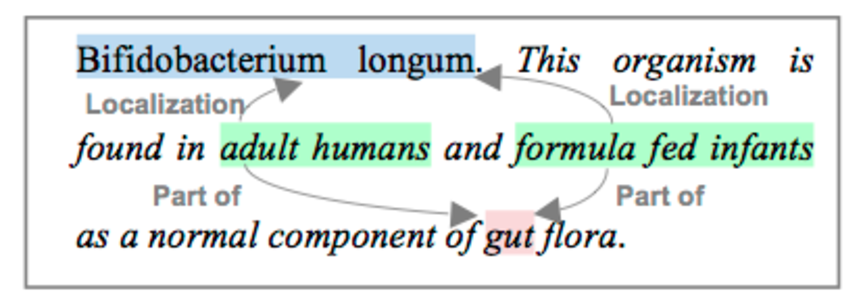
\includegraphics[scale=0.6]{figures/biotope.pdf}
 \caption{Example of event extraction task in BioNLP 2013 taks on bacteria biotope \citep{bossy2013bionlp}}
\label{fig:biotope}
\end{center}
\end{figure} 

The KYOTO\footnote{\url{http://kyoto-project.eu/}} (Knowledge Yielding Ontologies for Transition-based Organization) project developed a system that allows people in communities to define the meaning of their words and terms in a shared Wiki platform in a formal way \citep{Vossen2008}.
Part of the project was developing tools to automatically extract facts from large amounts of text and making these fact bases available.
One of the application domains was environmental science.
Figure~\ref{fig:kyoto} shows a graph representing facts extracted from a single sentence.
Several large sets of extracted facts can be downloaded, including those from publications by European Environment Agency and articles from the Journal of Environmental Biology.\EM{Kyoto deserves much more attention, but the website is such a mess that is hard to figure out the big picture.}  

\begin{figure}
\begin{center}
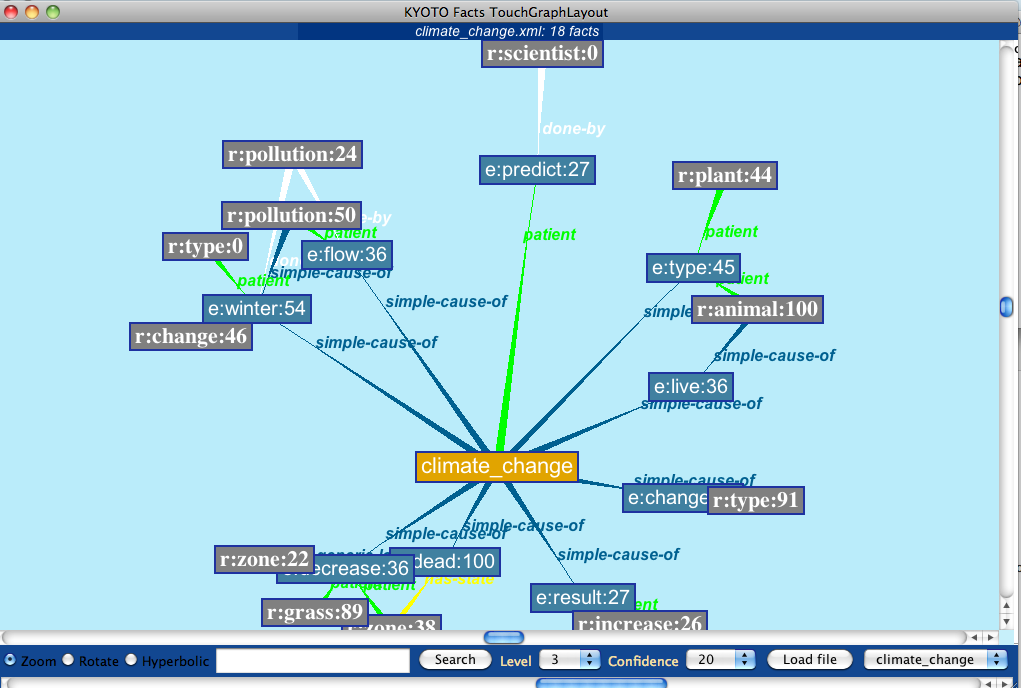
\includegraphics[scale=0.35]{figures/kyoto.png}
 \caption{Fact graph extracted by Kyoto system from the sentence ``Scientists predict that climate change could also cause a decrease in underwater grasses, more "dead zones" of low oxygen, more annual precipitation and a resulting increase in the flow of pollution, fewer wintering waterfowl, and a change in the types of plants and animals that live in the area.''}
\label{fig:kyoto}
\end{center}
\end{figure} 


GeoDeepDive\footnote{\url{http://hazy.cs.wisc.edu/hazy/geodeepdive}} is another text mining system for extracting information and knowledge from text, tables, and figures of geology journal articles \citep{Zhang2013GeoDeepDive}.
It combines data from several sources: unstructured data (hmtl documents, scanned papers, images), structured knowledge bases (Freebase, dictionaries), domain experts (expert rules and annotation) and crowds (annotation).
It performs extraction of entities (e.g., rock formations, locations, temporal intervals, etc.) and relations.
The goal is to support novel geological science, e.g., understanding the carbon cycle and characterizing the organic carbon content of Earth’s crust.
Figure~\ref{fig:geodeepdive} shows two examples of the user interface.
The top half shows a geographical representation of sample extraction throughout Northern America, where polygons represents a geological areas and their opacity indicates the number of extractions in that area.
The right hand side shows statistics such as total the number of units and measurements extracted from 36162 documents.
The bottom figure shows extractions for a particular rock formation (Barnett).
A table with measurements for Total Organic Carbon (TOC) is shown, together with the provenance, i.e. a the source text for the extraction.
Users are asked to provide feedback regarding the correctness of the extracted data, which is then used to improve the system.

A related project called PaleoDeepDive\footnote{\url{http://youtu.be/Cj2-dQ2nwoY}} has been started very recently.
It extracts fosil data -- such as biological classification, geographical distribution and geological location -- from journal arcticles and books on paleobiology.
One the aims is producing a more reliable biodiversity curve, which represents variation in the overal number of species over the past million of years.

\begin{figure}
\begin{center}
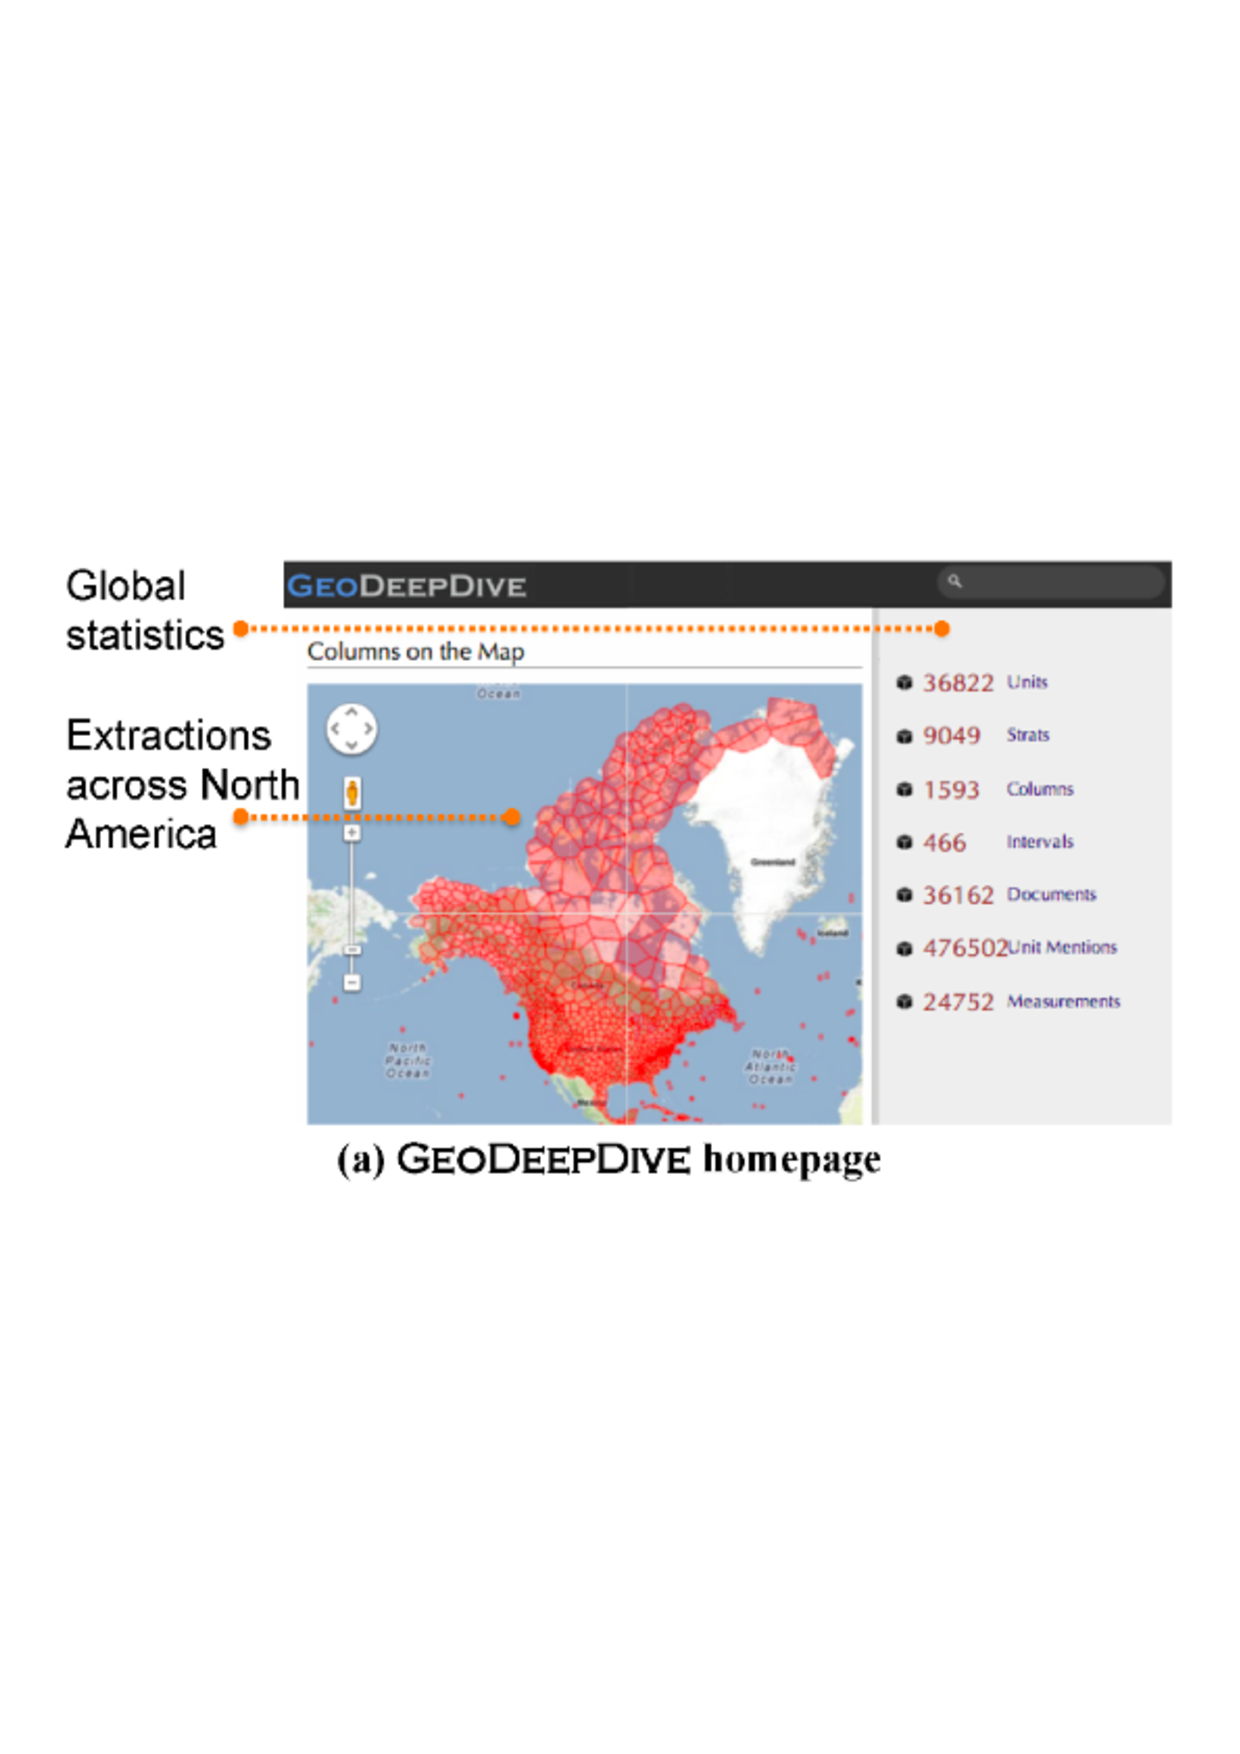
\includegraphics[scale=0.6]{figures/geodeepdive-1.pdf}
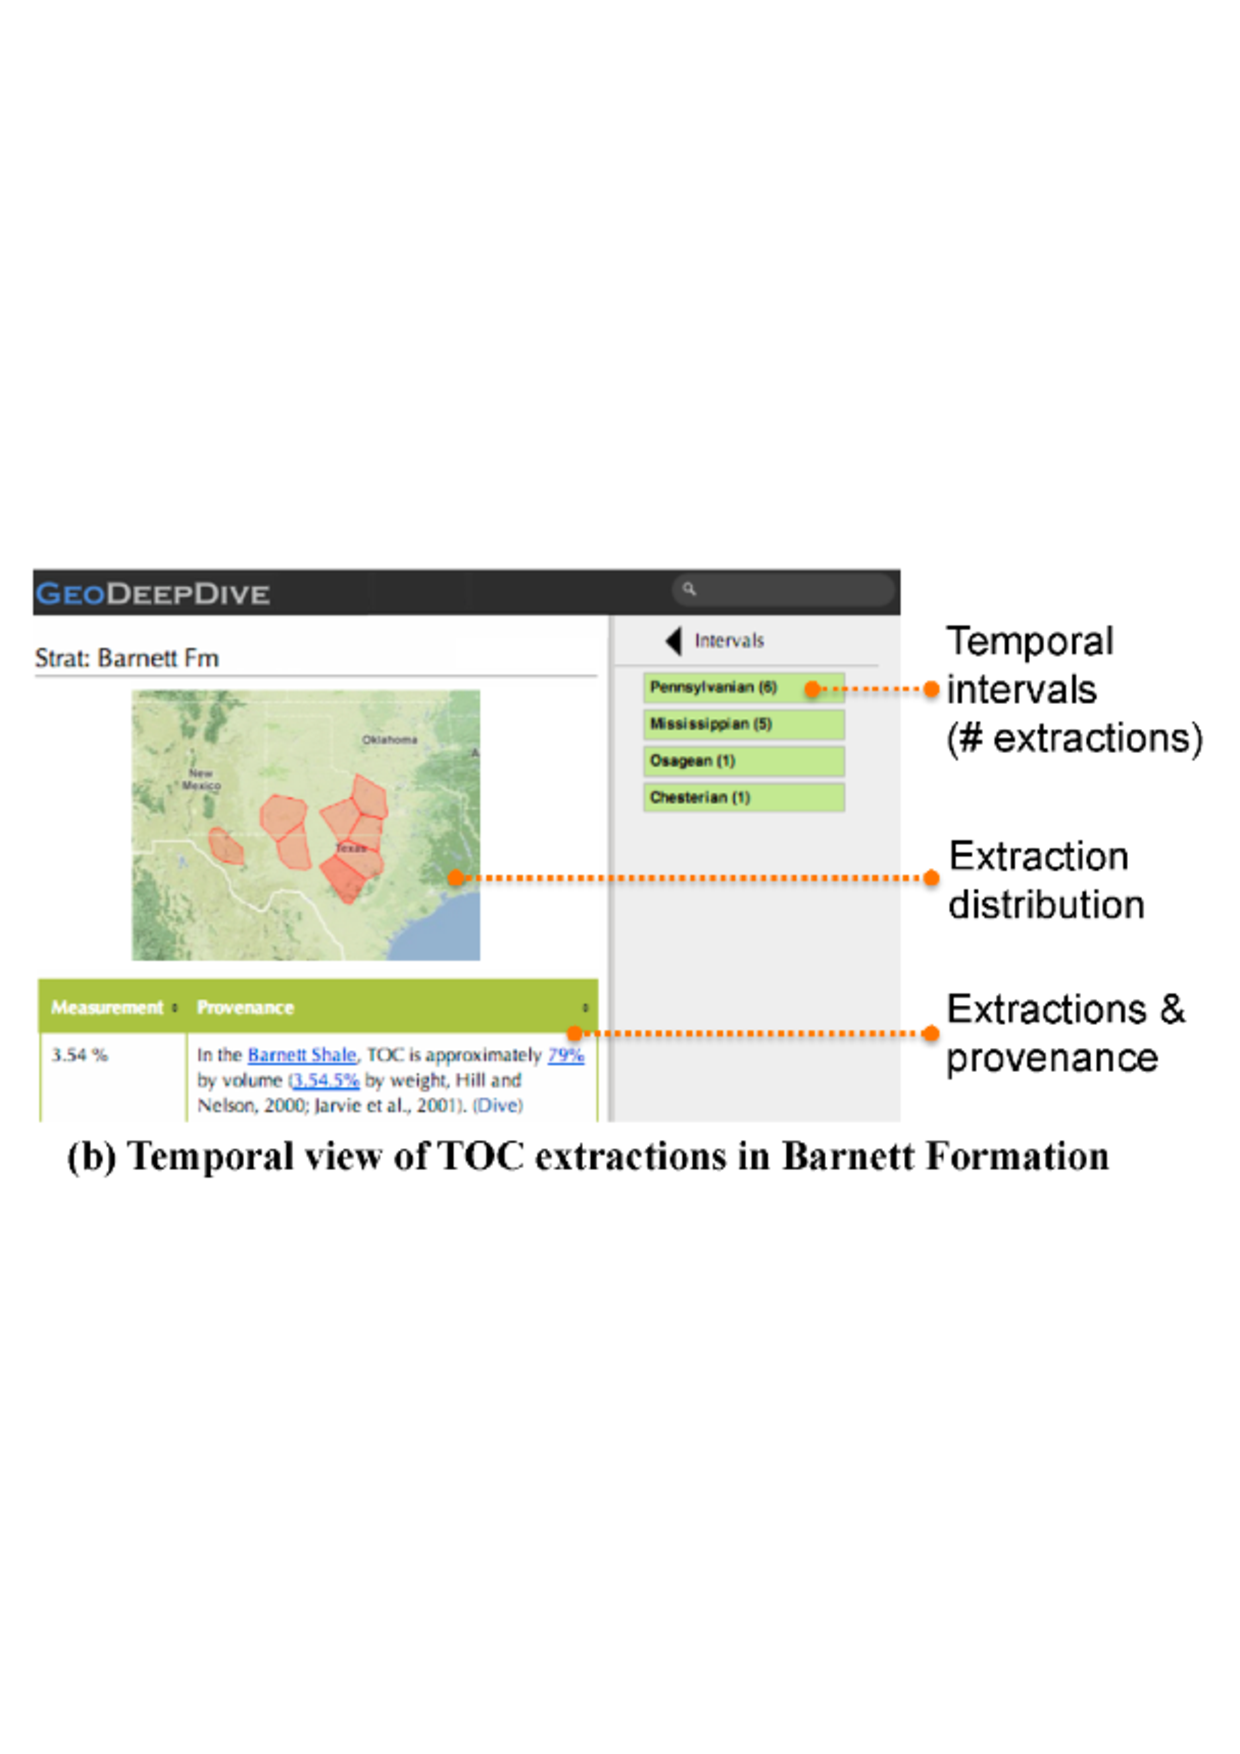
\includegraphics[scale=0.6]{figures/geodeepdive-2.pdf}
 \caption{GeoDeepDive user interface \citep{Zhang2013GeoDeepDive}}
\label{fig:geodeepdive}
\end{center}
\end{figure} 
   
In the area of ocean management, \citet{Ekstrom2008Exploratory} describe exploratory text mining of ocean law to measure overlapping jurisdictions of government agencies.  


%%% Local Variables: 
%%% mode: latex
%%% TeX-master: "ocwp1-d1"
%%% End: 